\documentclass{article}

\usepackage[inner=0.5cm,outer=0.5cm,top=1cm,bottom=0.5cm]{geometry}

\pagestyle{empty}
% This document contains the TikZ-header for all our LaTeX-computations.
% It especially contains all global graphic parameters.

\usepackage{amsmath, amssymb, amsfonts} % Standard Math-stuff

\usepackage{ifthen}

\usepackage{tikz}
\usetikzlibrary{calc}
\usetikzlibrary{positioning}
\usetikzlibrary{shapes}
\usetikzlibrary{patterns}


% Sometimes we want to implement different behaviour for the generated 
% HTML-pictures (for example, shading is not supported in HTML).
% For that we define a macro to check whether we run the code with
% htlatex. The code comes from 
% https://tex.stackexchange.com/questions/93852/what-is-the-correct-way-to-check-for-latex-pdflatex-and-html-in-the-same-latex
\makeatletter
\edef\texforht{TT\noexpand\fi
  \@ifpackageloaded{tex4ht}
    {\noexpand\iftrue}
    {\noexpand\iffalse}}
\makeatother


% Define a text=none option for nodes that ignores the given text, from
% https://tex.stackexchange.com/questions/59354/no-text-none-in-tikz
\makeatletter
\newif\iftikz@node@phantom
\tikzset{
  phantom/.is if=tikz@node@phantom,
  text/.code=%
    \edef\tikz@temp{#1}%
    \ifx\tikz@temp\tikz@nonetext
      \tikz@node@phantomtrue
    \else
      \tikz@node@phantomfalse
      \let\tikz@textcolor\tikz@temp
    \fi
}
\usepackage{etoolbox}
\patchcmd\tikz@fig@continue{\tikz@node@transformations}{%
  \iftikz@node@phantom
    \setbox\pgfnodeparttextbox\hbox{}
  \fi\tikz@node@transformations}{}{}
\makeatother

% Find the angle of a given line (within TikZ)
\newcommand{\tikzAngleOfLine}{\tikz@AngleOfLine}
\def\tikz@AngleOfLine(#1)(#2)#3{%
  \pgfmathanglebetweenpoints{%
    \pgfpointanchor{#1}{center}}{%
    \pgfpointanchor{#2}{center}}
  \pgfmathsetmacro{#3}{\pgfmathresult}%
}

% Now we define the global styles
% The global styles are defined nestedly. You have to give your tikzpicture
% the global options [vertexStyle, edgeStyle, faceStyle] to activate them.
% 
% You can disable labels by using the option nolabels, i.e. 
% vertexStyle=nolabels to deactivate vertex labels.
%
% If you want to have a specific style for your picture, you can also use
% this specific meta-style instead of the general style. For example if you
% want to use double edges in one single picture - no matter the style of
% the rest of the document - you can use edgeDouble instead of edgeStyle.
%
% To set the default style, modify the vertexStyle/.default entry.

% Vertex styles
\tikzset{ 
    vertexNodePlain/.style = {fill=#1, shape=circle, inner sep=0pt, minimum size=2pt, text=none},
    vertexNodePlain/.default=gray,
    vertexPlain/labels/.style = {
        vertexNode/.style={vertexNodePlain=##1},
        vertexLabel/.style={gray}
    },
    vertexPlain/nolabels/.style = {
        vertexNode/.style={vertexNodePlain=##1},
        vertexLabel/.style={text=none}
    },
    vertexPlain/.style = vertexPlain/#1,
    vertexPlain/.default=labels
}
\tikzset{
    vertexNodeNormal/.style = {fill=#1, shape=circle, inner sep=0pt, minimum size=4pt, text=none},
    vertexNodeNormal/.default = blue,
    vertexNormal/labels/.style = {
        vertexNode/.style={vertexNodeNormal=##1},
        vertexLabel/.style={blue}
    },
    vertexNormal/nolabels/.style = {
        vertexNode/.style={vertexNodeNormal=##1},
        vertexLabel/.style={text=none}
    },
    vertexNormal/.style = vertexNormal/#1,
    vertexNormal/.default=labels
}
\tikzset{
    vertexNodeBallShading/pdf/.style = {ball color=#1},
    vertexNodeBallShading/svg/.style = {fill=#1},
    vertexNodeBallShading/.code = {% Conditional shading depending whether we want pdf or svg output
        \if\texforht
            \tikzset{vertexNodeBallShading/svg=#1!90!black}
        \else
            \tikzset{vertexNodeBallShading/pdf=#1}
        \fi
    },
    vertexNodeBall/.style = {shape=circle, vertexNodeBallShading=#1, inner sep=2pt, outer sep=0pt, minimum size=3pt, font=\tiny},
    vertexNodeBall/.default = white,
    vertexBall/labels/.style = {
        vertexNode/.style={vertexNodeBall=##1, text=black},
        vertexLabel/.style={text=none}
    },
    vertexBall/nolabels/.style = {
        vertexNode/.style={vertexNodeBall=##1, text=none},
        vertexLabel/.style={text=none}
    },
    vertexBall/.style = vertexBall/#1,
    vertexBall/.default=labels
}
\tikzset{ 
    vertexStyle/.style={vertexNormal=#1},
    vertexStyle/.default = labels
}


% 1) optional: colour of vertex
% 2) position of the vertex
% 3) relative position of the node
% 4) name of the vertex
\newcommand{\vertexLabelR}[4][]{
    \ifthenelse{ \equal{#1}{} }
        { \node[vertexNode] at (#2) {#4}; }
        { \node[vertexNode=#1] at (#2) {#4}; }
    \node[vertexLabel, #3] at (#2) {#4};
}
% 1) optional: colour of vertex
% 2) position of the vertex
% 3) absolute position of the node
% 4) name of the vertex
\newcommand{\vertexLabelA}[4][]{
    \ifthenelse{ \equal{#1}{} }
        { \node[vertexNode] at (#2) {#4}; }
        { \node[vertexNode=#1] at (#2) {#4}; }
    \node[vertexLabel] at (#3) {#4};
}


% Edge styles
% If you have trouble with the double-lines overlapping, this might (?) help:
% https://tex.stackexchange.com/questions/288159/closing-the-ends-of-double-line-in-tikz
\newcommand{\edgeLabelColor}{blue!20!white}
\tikzset{
    edgeLineNone/.style = {draw=none},
    edgeLineNone/.default=black,
    edgeNone/labels/.style = {
        edge/.style = {edgeLineNone=##1},
        edgeLabel/.style = {fill=\edgeLabelColor,font=\small}
    },
    edgeNone/nolabels/.style = {
        edge/.style = {edgeLineNone=##1},
        edgeLabel/.style = {text=none}
    },
    edgeNone/.style = edgeNone/#1,
    edgeNone/.default = labels
}
\tikzset{
    edgeLinePlain/.style={line join=round, draw=#1},
    edgeLinePlain/.default=black,
    edgePlain/labels/.style = {
        edge/.style={edgeLinePlain=##1},
        edgeLabel/.style={fill=\edgeLabelColor,font=\small}
    },
    edgePlain/nolabels/.style = {
        edge/.style={edgeLinePlain=##1},
        edgeLabel/.style={text=none}
    },
    edgePlain/.style = edgePlain/#1,
    edgePlain/.default = labels
}
\tikzset{
    edgeLineDouble/.style = {very thin, double=#1, double distance=.8pt, line join=round},
    edgeLineDouble/.default=gray!90!white,
    edgeDouble/labels/.style = {
        edge/.style = {edgeLineDouble=##1},
        edgeLabel/.style = {fill=\edgeLabelColor,font=\small}
    },
    edgeDouble/nolabels/.style = {
        edge/.style = {edgeLineDouble=##1},
        edgeLabel/.style = {text=none}
    },
    edgeDouble/.style = edgeDouble/#1,
    edgeDouble/.default = labels
}
\tikzset{
    edgeStyle/.style = {edgePlain=#1},
    edgeStyle/.default = labels
}

% Face styles
% Here we have an exception - the style face is always defined.
% 
\newcommand{\faceColorY}{yellow!60!white}   % yellow
\newcommand{\faceColorB}{blue!60!white}     % blue
\newcommand{\faceColorC}{cyan!60}           % cyan
\newcommand{\faceColorR}{red!60!white}      % red
\newcommand{\faceColorG}{green!60!white}    % green
\newcommand{\faceColorO}{orange!50!yellow!70!white} % orange

% define default face colour (and default swap colour)
\newcommand{\faceColor}{\faceColorY}
\newcommand{\faceColorSwap}{\faceColorC}

% define secondary default colours (to use in a single section)
\newcommand{\faceColorFirst}{green!40!white}
\newcommand{\faceColorSecond}{gray!15!white}
\newcommand{\faceColorThird}{red!17!white}
\newcommand{\faceColorFourth}{olive!20!white}

\tikzset{
    face/.style = {fill=#1},
    face/.default = \faceColor,
    faceY/.style = {face=\faceColorY},
    faceB/.style = {face=\faceColorB},
    faceC/.style = {face=\faceColorC},
    faceR/.style = {face=\faceColorR},
    faceG/.style = {face=\faceColorG},
    faceO/.style = {face=\faceColorO}
}
\tikzset{
    faceStyle/labels/.style = {
        faceLabel/.style = {}
    },
    faceStyle/nolabels/.style = {
        faceLabel/.style = {text=none}
    },
    faceStyle/.style = faceStyle/#1,
    faceStyle/.default = labels
}
\tikzset{ face/.style={fill=#1} }
\tikzset{ faceSwap/.code=
    \ifdefined\swapColors
        \tikzset{face=\faceColorSwap}
    \else
        \tikzset{face=\faceColor}
    \fi
}



\usepackage{hyperref}


\begin{document}



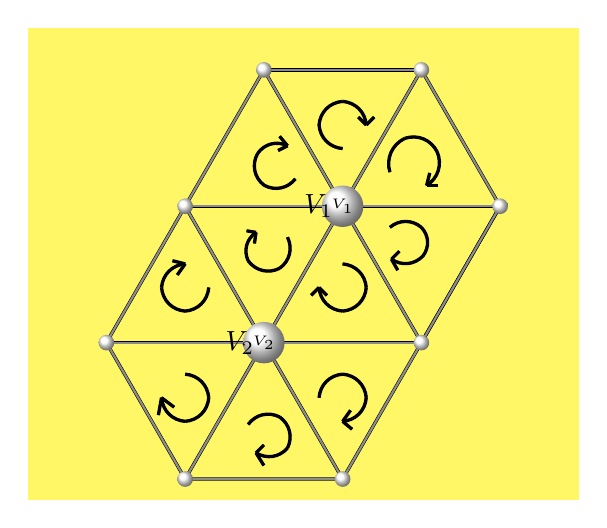
\begin{tikzpicture}[vertexBall, edgeDouble, faceStyle, scale=2]

% Define the coordinates of the vertices
\coordinate (V1_1) at (0, 0);
\coordinate (V2_1) at (1, 0);
\coordinate (V3_1) at (0.4999999999999999, 0.8660254037844386);
\coordinate (V4_1) at (1.5, 0.8660254037844388);
\coordinate (V5_1) at (-0.5, 0.8660254037844388);
\coordinate (V6_1) at (2*0.4999999999999999, 2*0.8660254037844386);
\coordinate (V7_1) at (0, 2*0.8660254037844386);

\coordinate (V8_1) at (0.5, 2*0.8660254037844386-0.2);
\coordinate (V9_1) at (0.5, 2*0.8660254037844386-0.5);
\coordinate (V10_1) at (0.35, 2*0.8660254037844386-0.35);
\coordinate (V11_1) at (0.65, 2*0.8660254037844386-0.35);
\coordinate (V12_1) at (0.6, 2*0.8660254037844386-0.3);
\coordinate (V13_1) at (0.7, 2*0.8660254037844386-0.3);

\coordinate (V8_3) at (0.5, 0.2);
\coordinate (V9_3) at (0.5,0.5);
\coordinate (V10_3) at (0.35, 0.35);
\coordinate (V11_3) at (0.65, 0.35);
\coordinate (V12_3) at (0.3, 0.3);
\coordinate (V13_3) at (0.4, 0.3);

\coordinate (V8_2) at (1.25, 2*0.8660254037844386-0.2);
\coordinate (V9_2) at (0.5, 2*0.8660254037844386-0.5);
\coordinate (V10_2) at (0.35, 2*0.8660254037844386-0.35);
\coordinate (V11_2) at (0.65, 2*0.8660254037844386-0.35);
\coordinate (V12_2) at (0.6, 2*0.8660254037844386-0.3);
\coordinate (V13_2) at (0.7, 2*0.8660254037844386-0.3);
%%%%%%%%%%%%%%%%%%%%%%%%
\coordinate (h11) at (0.5 +0.4*0.75,0.8660+0.5*0.433);
\coordinate (h21) at (0.5 +0.8*0.75,0.8660+0.8*0.433);
\coordinate (h31) at (0.5 +0.7*0.75-0.433*0.3,0.8660+0.65*0.433+0.75*0.2);
\coordinate (h41) at (0.5 +0.7*0.7+0.433*0.1,0.8660+0.65*0.433-0.75*0.2);
\coordinate (h51) at (0.5 +0.7*0.7+0.433*0.1+0.07,0.8660+0.65*0.433-0.75*0.2);
\coordinate (h61) at (0.5 +0.7*0.7+0.433*0.1+0.02,0.8660+0.65*0.433-0.75*0.2+0.08);

\coordinate (h12) at (0.15,0.6695);
\coordinate (h22) at (-0.1,0.5196);
\coordinate (h32) at (0.1,0.8660-0.65*0.433-0.75*0.15);
\coordinate (h42) at (-0.05,0.7);
\coordinate (h52) at (-0.06-0.05,0.7+0.01);
\coordinate (h62) at (-0.02-0.04,0.7-0.07);

\coordinate (h13) at (0.2,1.04);
\coordinate (h23) at (0.2-0.8*0.3,0.866+0.8*0.444-0.02);
\coordinate (h33) at (-0.0,1.0);
\coordinate (h43) at (0.15,1.25);
\coordinate (h53) at (0.15-0.05,1.25+0.06);
\coordinate (h63) at (0.15-0.06,1.25-0.03);

\coordinate (h14) at (0.8,0.732);
\coordinate (h24) at (1.01,0.55);
\coordinate (h34) at (1.0,0.732);
\coordinate (h44) at (0.81,0.53);
\coordinate (h54) at (0.81+0.05,0.53+0.05);
\coordinate (h64) at (0.81+0.04,0.53-0.07);
%\coordinate (h12) at (0.5 -0.5*0.75,0.8660-0.5*0.433);
%\coordinate (h13) at (0.5 -0.5*0.75,0.8660-0.5*0.433+2*0.2165);
%\coordinate (h14) at (0.5 +0.5*0.75,0.8660-0.5*0.433);

%\coordinate (h22) at (0.5 -0.8*0.75,0.8660-0.8*0.433);
%\coordinate (h23) at (0.5 -0.8*0.75,0.8660+0.8*0.433);
%\coordinate (h24) at (0.5 +0.8*0.75,0.8660-0.8*0.433);
\coordinate (V2_2) at (.5, -0.866);
\coordinate (V5_2) at (-1., 0);
\coordinate (V6_2) at (-0.4999999999999999, -0.8660254037844386);

\coordinate (V8_4) at (0.5, -0.2);
\coordinate (V9_4) at (0.5,-0.5);
\coordinate (V10_4) at (0.35, -0.35);
\coordinate (V11_4) at (0.65, -0.35);
\coordinate (V12_4) at (0.56, -0.55);
\coordinate (V13_4) at (0.55, -0.43);

\coordinate (V8_5) at (-0.5, -0.2);
\coordinate (V9_5) at (-0.5,-0.5);
\coordinate (V10_5) at (-0.35, -0.35);
\coordinate (V11_5) at (-0.65, -0.35);
\coordinate (V12_5) at (-.67, -0.46);
\coordinate (V13_5) at (-0.57, -0.41);

\coordinate (ha12) at (0.15,-0.6695);
\coordinate (ha22) at (-0.1,-0.5196);
\coordinate (ha32) at (0.1,-0.8660+0.65*0.433+0.75*0.15);
\coordinate (ha42) at (-0.05,-0.7);
\coordinate (ha52) at (-0.0,-0.78);
\coordinate (ha62) at (-0.0,-0.7+0.05);

\coordinate (V8_6) at (-0.5, 0.2);
\coordinate (V9_6) at (-0.5,0.5);
\coordinate (V10_6) at (-0.35, 0.35);
\coordinate (V11_6) at (-0.65, 0.35);
\coordinate (V12_6) at (-0.58, 0.52);
\coordinate (V13_6) at (-0.55, 0.43);

%\coordinate (t1) at (-0.,.433);
%\coordinate (t2) at (-0.,.433);
% Fill in the faces
\fill[face] (2,2) -- (2,-1) --(-1.5,-1) -- (-1.5,2) -- cycle;
\fill[face]  (V2_1) -- (V3_1) -- (V1_1) -- cycle;
%\node[faceLabel] at (barycentric cs:V2_1=1,V3_1=1,V1_1=1) {$F_3$};
\fill[face]  (V2_1) -- (V4_1) -- (V3_1) -- cycle;
%\node[faceLabel] at (barycentric cs:V2_1=1,V4_1=1,V3_1=1) {$F_2$};
\fill[face] (V5_1) -- (V3_1) -- (V1_1) --cycle;
%\node[faceLabel] at (barycentric cs:V5_1=1,V3_1=1,V1_1=1) {$F_4$};
\fill[face] (V6_1) -- (V3_1) -- (V4_1) --cycle;
%\node[faceLabel] at (barycentric cs:V6_1=1,V7_1=1,V3_1=1) {$F_6$};
%\node[faceLabel] at (barycentric cs:V5_1=1,V7_1=1,V3_1=1) {$F_5$};
%\node[faceLabel] at (barycentric cs:V6_1=1,V3_1=1,V4_1=1) {$F_1$};

%\node[faceLabel] at (barycentric cs:V5_2=1,V5_1=1,V1_1=1) {$F$};
%\node[faceLabel] at (barycentric cs:V5_2=1,V6_2=1,V1_1=1) {$F_9$};
%\node[faceLabel] at (barycentric cs:V6_2=1,V2_2=1,V1_1=1) {$F_8$};
%\node[faceLabel] at (barycentric cs:V2_1=1,V2_2=1,V1_1=1) {$ $};
% Draw the edges
%\draw[edge] (t2) --  (t1);
\draw[edge] (V2_1) --  (V1_1);
\draw[edge] (V1_1) --   (V3_1);
\draw[edge] (V3_1) --  (V2_1);
\draw[edge] (V4_1) --   (V2_1);
\draw[edge] (V3_1) --   (V4_1);
\draw[edge] (V3_1) --   (V6_1);
\draw[edge] (V6_1) --  (V4_1);
\draw[edge] (V3_1) --   (V5_1);
\draw[edge] (V1_1) --   (V5_1);
\draw[edge] (V7_1) --  (V6_1);
\draw[edge] (V7_1) --  (V5_1);
\draw[edge] (V7_1) --  (V3_1);

\draw[edge=black] (V11_1) --  (V12_1);
\draw[edge=black] (V11_1) --  (V13_1);
%\draw[edge] (V9_1) to[bend left=90]  (V8_1);
%\draw[edge] (V9_1) to[bend right=90]  (V8_1);
\draw[edge=black] (V9_1) to[bend left=40]  (V10_1);
\draw[edge=black] (V8_1) to[bend right=40]  (V10_1);
\draw[edge=black] (V8_1) to[bend left=40]  (V11_1);

\draw[edge=black] (V10_3) --  (V12_3);
\draw[edge=black] (V10_3) --  (V13_3);
%\draw[edge] (V9_1) to[bend left=90]  (V8_1);
%\draw[edge] (V9_1) to[bend right=90]  (V8_1);
\draw[edge=black] (V9_3) to[bend left=40, black]  (V11_3);
\draw[edge=black] (V8_3) to[bend left=40]  (V10_3);
\draw[edge=black] (V8_3) to[bend right=40]  (V11_3);

\draw[edge=black] (h11) to[bend left=40]  (h31);
\draw[edge=black] (h21) to[bend right=40]  (h31);
\draw[edge=black] (h21) to[bend left=40]  (h41);
\draw[edge=black] (h51) to  (h41);
\draw[edge=black] (h61) to  (h41);

%\draw[edge] (h12) to[bend left=40]  (h32);
\draw[edge=black] (h22) to[bend right=40]  (h32);
\draw[edge=black] (h12) to[bend left=40]  (h32);
\draw[edge=black] (h22) to[bend left=40]  (h42);
\draw[edge=black] (h62) to  (h42);
\draw[edge=black] (h52) to  (h42);
%\draw[edge] (h12) to[bend left=40]  (h32);
\draw[edge=black] (h23) to[bend right=40]  (h33);
\draw[edge=black] (h13) to[bend left=40]  (h33);
\draw[edge=black] (h23) to[bend left=40]  (h43);
\draw[edge=black] (h53) to  (h43);
\draw[edge=black] (h63) to  (h43);

\draw[edge=black] (h24) to[bend right=40]  (h34);
\draw[edge=black] (h14) to[bend left=40]  (h34);
\draw[edge=black] (h24) to[bend left=40]  (h44);
\draw[edge=black] (h54) to  (h44);
\draw[edge=black] (h64) to  (h44);
%\draw[edge] (h14) to[bend left=90]  (h24);


\draw[edge] (V2_2) --   (V1_1);
\draw[edge] (V4_1) --   (V2_2);
\draw[edge] (V1_1) --   (V6_2);
\draw[edge] (V6_2) --   (V5_2);
\draw[edge] (V6_2) --   (V2_2);
\draw[edge] (V5_2) --   (V5_1);
\draw[edge] (V1_1) --   (V5_2);



\draw[edge=black] (V9_4) --  (V12_4);
\draw[edge=black] (V9_4) --  (V13_4);
%\draw[edge] (V9_1) to[bend left=90]  (V8_1);
%\draw[edge] (V9_1) to[bend right=90]  (V8_1);
\draw[edge=black] (V9_4) to[bend right=40, black]  (V11_4);
\draw[edge=black] (V8_4) to[bend right=40]  (V10_4);
\draw[edge=black] (V8_4) to[bend left=40]  (V11_4);


\draw[edge=black] (V11_5) --  (V12_5);
\draw[edge=black] (V11_5) --  (V13_5);
%\draw[edge] (V9_1) to[bend left=90]  (V8_1);
%\draw[edge] (V9_1) to[bend right=90]  (V8_1);
\draw[edge=black] (V9_5) to[bend right=40, black]  (V10_5);
\draw[edge=black] (V9_5) to[bend left=40, black]  (V11_5);
\draw[edge=black] (V8_5) to[bend left=40]  (V10_5);
%\draw[edge=black] (V8_5) to[bend right=40]  (V11_5);

\draw[edge=black] (ha22) to[bend left =40]  (ha32);
\draw[edge=black] (ha12) to[bend left=40]  (ha42);
\draw[edge=black] (ha12) to[bend right=40]  (ha32);
%\draw[edge=black] (ha22) to[bend right=40]  (ha42);
\draw[edge=black] (ha62) to  (ha42);
\draw[edge=black] (ha52) to  (ha42);
%%%%%%%%%%%%%%%%%%%%%%%%%%%%%%%%%%%%%%%%%%%%%%%%%%%%%
\draw[edge=black] (V9_6) --  (V12_6);
\draw[edge=black] (V9_6) --  (V13_6);
%\draw[edge] (V9_1) to[bend left=90]  (V8_1);
%\draw[edge] (V9_1) to[bend right=90]  (V8_1);
\draw[edge=black] (V9_6) to[bend right=40]  (V11_6);
\draw[edge=black] (V8_6) to[bend right=40]  (V10_6);
\draw[edge=black] (V8_6) to[bend left=40]  (V11_6);
%%%%%%%%%%%%%%%%%%%%%%%%%%%%%%%%%%%%%%%%%%%%%%%%%%%%
% Draw the vertices
\vertexLabelR{V1_1}{left}{$V_2$}
\vertexLabelR{V2_1}{left}{$ $}
\vertexLabelR{V3_1}{left}{$V_1$}
\vertexLabelR{V4_1}{left}{$ $}
\vertexLabelR{V5_1}{left}{$ $}
\vertexLabelR{V6_1}{left}{$ $}
\vertexLabelR{V7_1}{left}{$ $}
%\vertexLabelR{h11}{left}{$1$}
%\vertexLabelR{h12}{left}{$2$}
%\vertexLabelR{h32}{left}{$3$}
%\vertexLabelR{h14}{left}{$4$}
%\vertexLabelR{h15}{left}{$ $}
%\vertexLabelR{h21}{left}{$1$}
%\vertexLabelR{h22}{left}{$2$}
%\vertexLabelR{h23}{left}{$3$}
%\vertexLabelR{h24}{left}{$4$}

\vertexLabelR{V2_2}{left}{$ $}
\vertexLabelR{V5_2}{left}{$ $}
\vertexLabelR{V6_2}{left}{$ $}
\end{tikzpicture}
\end{document}
